\documentclass[12pt]{article}
 
\usepackage[margin=1in]{geometry} 
\usepackage{graphicx}
\usepackage{url}
\usepackage{hyperref}
\usepackage{float}
\usepackage{quoting}

\usepackage{baskervald}
 
\newif\iffull
\fulltrue % comment out to hide answers
\begin{document}
 
\title{Stargazer Xeru}
\date{}

\maketitle
\begin{figure}[!htb]
  \centering
  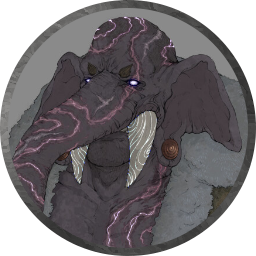
\includegraphics[width=.7\textwidth]{./resources/Stargazer_Xeru}
  \caption{Stargazer Xeru's current appearance.}
\end{figure}

\clearpage

\section{Character Description}

As a Loxodon, Xeru would be a unique visual no matter where he went, but the
angry purple scars that layer his entire body ensure he's remembered where he
passes. At a prodigous 362 years old, Xeru sports large droopy ears, faded skin
and tusks, although the tusks themselves are engraved with some sort of
intricate tribal markings, mirroring his scars. But most people have to look up
to see them, as he stands a striking 8' tall. Given his size, most of his
clothes have to be tailor made, which combined with his unfortutely empty coin
purse, results in him having the one open chested fur cloak, which he always
wears. The cloak is well-made and maintained, dyed a pale green and upon close
inspection has chain-mail hidden underneath. This is mostly redundant, as his
leathery hide turns equally many blows away.

None of this is quite as striking as the maul he holds, as tall as he is,
brutally heavy; Xeru can look quite menacing to the casual observer. However,
those who would speak to him would find him well-mannered and friendly,
especially when sharing a drink... which he does often. Xeru unfortunately has
a bit of a drinking problem, which explains where all his gold seems to
dissapear to when you think about how much alcohol it would take to get a 8'
half-ton elephant drunk. Luckily, Xeru comes prepared for any occasion, hauling
many kegs of ale around with him on his travels, brews he favored across the
lands. He only shares those ales with those he considers family which for now is
just Varkos, his only real companion here in Dead King's Bay.

\begin{figure}[H]
  \centering
  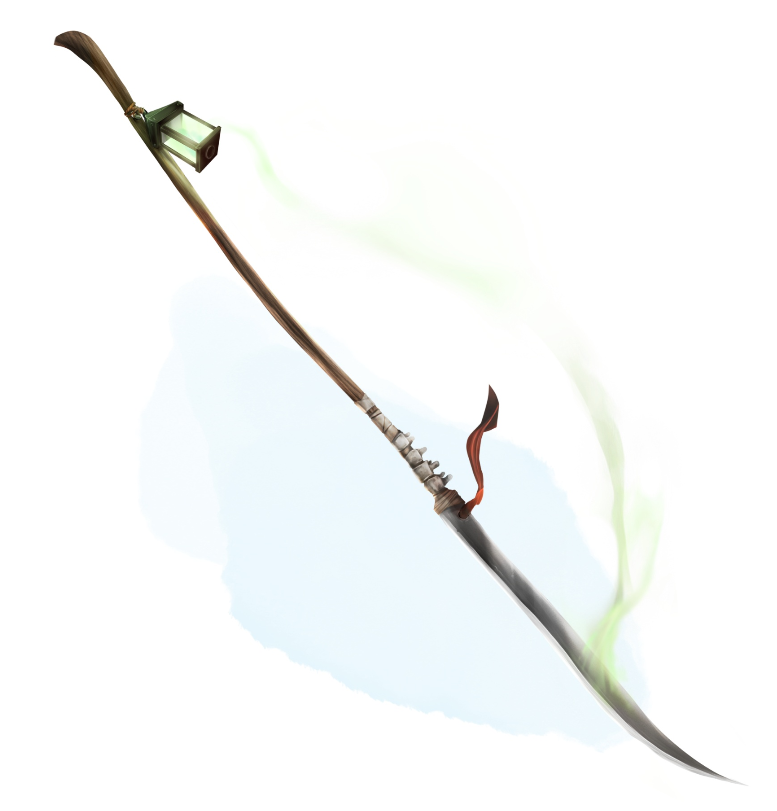
\includegraphics[width=.5\textwidth]{./resources/glaive}
  \caption{Xeru's Glaive.}
\end{figure}

\iffull
  \section{Backstory}

  \subsection{The Kerun Clan}

  \subsection{A Desperate Doctor}

  \subsection{Betrayal}
  
  \subsection{Stargazer Xeru}

  \section{Related NPCs}

  \section{Notes for the DM}
  \begin{itemize}
    \item \textbf{\textit{The Kerun Clan}}:
      \begin{itemize}
        \item The clan from which Xeru hailed, they settled 500 years ago from
          the current date on the Eastern border of The Kingdom of Valdir
          Descent.
        \item Afflicted with a magical genetic disease/curse which the clan
          called \textit{Scarring}. It causes horrific purple scars and often
          claims the lives of it's victims, but has somehow been incorporated as
          a rite of adulthood by the clan.
        \item Xeru spent the first 100 years of his life watching as he and
          others of his family were claimed by it. He decided to dedicate his
          life to finding a cure and traveled to \textit{XUniversity} to study
          medicine.
      \end{itemize}
    \item \textbf{\textit{Xuniversity}}: 
      \begin{itemize}
        \item Xeru arrived at the university destitute and clueless, but chance led
          him to make a friend named \textit{Cyrus Drayden}, a youth decended from
          the local governer, \textit{Lord Drayden}.
        \item With his aid and influence, they both enrolled in the college and
          over the next 30 years became relatively well known authorities on the
          subject of magical diseases.
        \item After 30 years of the disease eluding him, Xeru discovered to his
          horror that the \textit{Scarring} had been recorded to be caused by
          a curse an ancient lich had laid upon the land before he fell in the
          exact area where his clan had settled.
        \item It was recorded that the curse drained the life of the afflicted
          to empower the lich.
        \item The lich's name was \textit{Azuch}.
      \end{itemize}
    \item \textbf{Betrayal}:
      \begin{itemize}
        \item Horrified by the truth, he confided in his only friend Cyrus what
          was going on, and begged him to help move his tribe away from the
          land. Cyrus agreed, and told Xeru not to worry.
        \item However, in the middle of that night, Xeru recieved a desperate
          message from a sending spell from the tribe elder, of how guards from
          \textit{Drayden} manor were massacring the village.
        \item In his furious alarm, Xeru stormed his way into the
          \textit{Drayden} estate, knocking out but not killing the few guards.
          Finding \textit{Cyrus}, his friend tearfully explained that he had no
          other choice, that he could not allow such an ancient power to
          possibly rise again, and furthermore could not allow anyone to know
          that the lich was still active, lest his followers rally.
          \textit{Cyrus} then ordered his guards to capture Xeru.
        \item Consumed by bitter hatred by the betrayal of his best friend, Xeru
          picked up a halberd from a fallen guard and cut his way out of his
          encirclement, killing for the first time in his life. He fled to the
          night leaving a wake of carnage in \textit{Drayden manor}.
      \end{itemize}
    \item \textbf{Aftermath and Wandering}:
      \begin{itemize}
        \item Immediately after he left, \textit{Lord Drayden} placed a massive
          bounty of 10,000 gold pieces on his head, claiming the charges of Mass
          Murder, destruction of his estate, and treason. He was wanted dead, or
          alive. Alive would be worth an extra 5,000 gold pieces.
        \item Xeru traveled back to his village and found it under strict guard,
          with no Loxodon in sight, atleast not living ones.
        \item Afterwards, Xeru spent the next 200 years of his life aimlessly
          wandering and fleeing from his bounty hunters. He made a few coin here
          and there acting as a doctor until eventually he was forced to attempt
          a suicidal journey into a horrifically dangerous pass that would lead
          into the \textit{Wolvine} territory, in an attempt to elude his
          hunters once and for all.
        \item He would have died 100 times over in the pass, but either through
          luck or some kind of supernatural force, he was unharmed in his
          passage. A star that shined faintly in the sky, which coincidentally
          always seemed to lead in the correct direction. Xeru pays homage to
          \textit{NavigationGod} because of this, as he attributes his survival
          to her.
        \item After entering the Wolvine kingdom, the star continued to lead
          Xeru, eventually landing him in Dead Kings Bay before dissapearing
          without a sight. He now resides there, posing as a old war veteran and
          doing some medicine and cartography work, a job he picked up after his
          supposed encounter with \textit{NavigationGod}.
      \end{itemize}
  \end{itemize}
\fi

\end{document}
